\documentclass[12pt,a4paper]{article}

\input{../preamble_files/packages}
\input{../preamble_files/figures}
\input{../preamble_files/references}
\input{../preamble_files/shortcuts}
\input{../preamble_files/listings}

\pagestyle{fancy}
\lhead{Richard Whitehill}
\chead{MATH 551 -- HW 4}
\rhead{04/21/22}
\cfoot{\thepage~of~\pageref{LastPage}}

\newcommand{\prob}[2]{\textbf{#1)} #2}

\setlength{\parskip}{\baselineskip}
\setlength{\parindent}{0pt}

\begin{document}

\prob{1}{Consider the function
\begin{align*}
    f(x) = \frac{1}{1 + 25 x^2}
.\end{align*}
on the interval $\left[ -1,1 \right]$.
}

a) For $n = 5,\,10,\,20$ plot the error $e(x) = f(x) - p_{n}(x)$ where the polynomial $p_{n}(x)$ is computed by interpolating at the $n+1$ equally-spaced nodes over $[-1,1]$.

The code for interpolation is recycled from the previous homework.
Again, we perform Lagrange interpolation since it is the most straightforward to program, and there is no clear advantage to using divided differences.
A script for the interpolation and generation of data points is shown below.
The program also addresses parts (b) and (c) of this question.

\inputpython{./prob4.py}

\begin{figure}[H]
    \begin{center}
        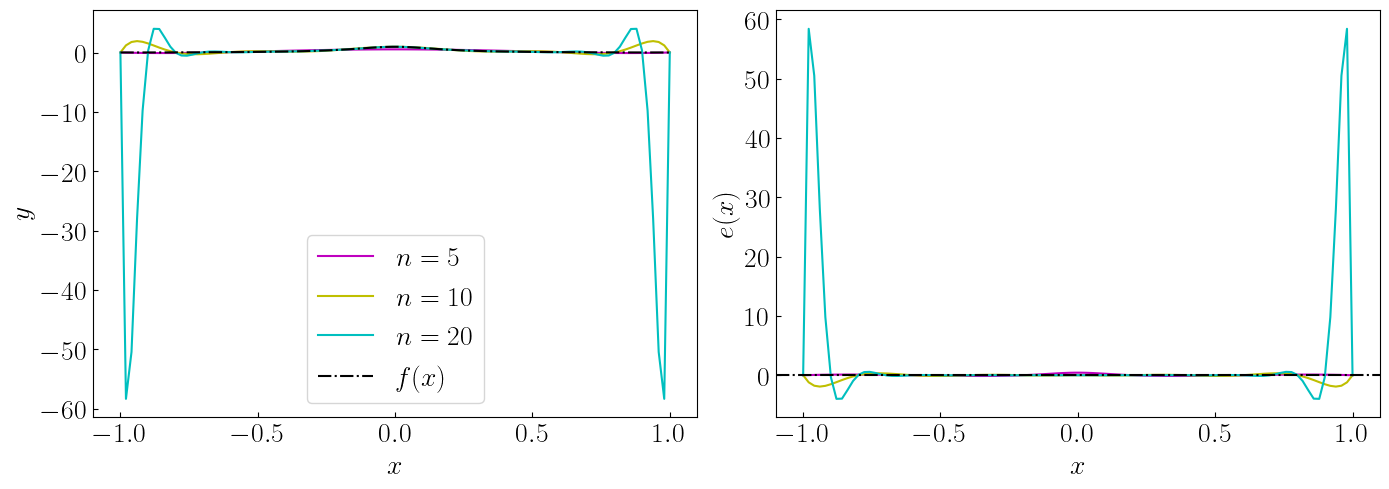
\includegraphics[scale=0.45]{./fig1.png} 
    \end{center}
\end{figure}

b) Describe what you observe numerically in (a) and Google \textbf{Runge's phenomenon} to study the reason.

It is seen that as the degree of the polynomial becomes larger, the interpolation becomes less stable at the end points.
That is, the polynomial develops a stronger oscillating behavior in order to match at the increasing number of nodes.
At the end points this leads to larger values in the function evaluation since the maximum error, which is proportional to $f^{\left( n+1 \right)}(\xi)$, becomes unbounded.

c) Repeat Part (a) but interpolate at the $n+1$ Chebyshev nodes over $[-1,1]$.
Describe what you observe numerically.

The Lagrange interpolation is repeated using Chebyshev nodes on the given interval:
\begin{align*}
    x_{j} = \frac{a+b}{2} + \frac{b-a}{2}\cos{\left[ \frac{\left( 2j+1 \right)\pi}{2\left( n+1 \right)} \right]}
.\end{align*}
for $j = 0,\,1,\ldots,\,n$.

It is clear that the interpolation is more stable across the entire interval.
This is because the points become closer together at the end points, meaning that the function cannot vary as much at the boundaries.
That is, the error term does not become unbounded since the derivatives are not as large.

A plot of the distribution of $x$ data points is shown below the interpoation to illustrate the difference between the Chebyshev distribution against the uniform distribution of points.

\begin{figure}[H]
    \begin{center}
        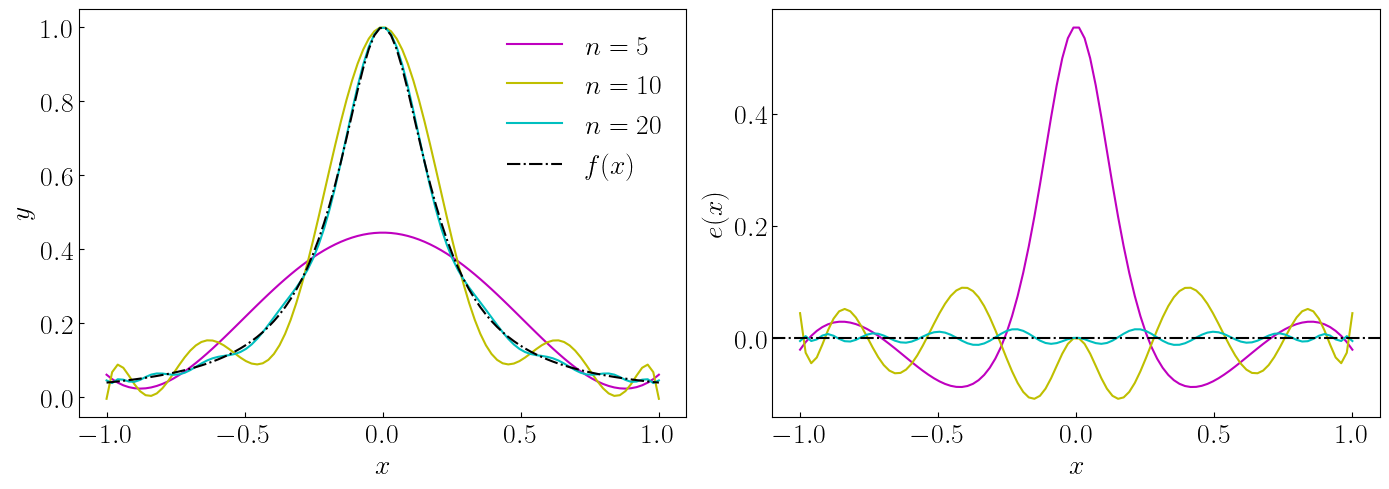
\includegraphics[scale=0.45]{./fig2.png} 
    \end{center}
\end{figure}

\begin{figure}[H]
    \begin{center}
        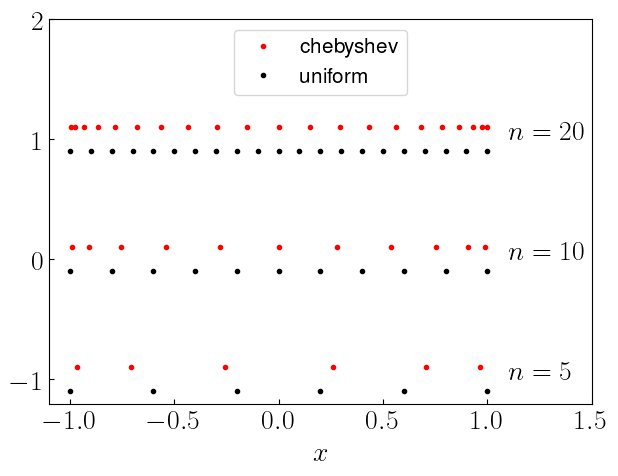
\includegraphics[scale=0.75]{./fig3.png} 
    \end{center}
\end{figure}

\prob{2}{Find one picture with some object and reconstruct the shape with cubic spline reconstruction.}

For this problem, I used the cubic spline code, translated into python, to reproduce the top outline on the yoshi (insert super mario bros sound effect here!) image below.
It is seen that the cubic spine reconstruction is fairly good.
That is, it generally matches the shape of the curve, but since spline fits are meant to possess a high degree of smoothness, it does not inherit the cusps (i.e. the places where the derivative is discontinuous) of the original image.

\begin{figure}[H]
    \begin{center}
        
\includegraphics[scale=0.3]{./yoshi.jpg} 
    \end{center}
\end{figure}

\begin{figure}[H]
    \begin{center}
        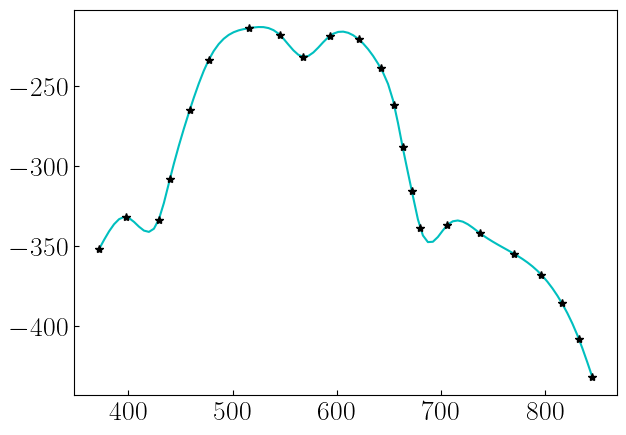
\includegraphics[scale=0.75]{./fig4.png} 
    \end{center}
\end{figure}

\inputpython{./prob5.py}

\end{document}
